\documentclass[12pt]{article}
\usepackage{amsmath}
\usepackage{amssymb}
\usepackage{tikz}
\usepackage{circuitikz}
\usepackage{tkz-euclide}
\usepackage{pgfplots}
\usepackage[many]{tcolorbox}
\tikzset{european}
\pgfplotsset{compat=1.18}
\usepgfplotslibrary{fillbetween}
\newtcolorbox{BOX}{
colframe=white,
colback=white,
enhanced,
boxrule=1.5pt,
borderline={0.75pt}{0pt}{dashed},
}


\title{Calculus}
\author{Hertzberg, Joakim D.}
\date{\today}
\begin{document}
\maketitle
\begin{center}
MAT03c: Mathematics 3c
\vfill
This document uses \LaTeX\ in combination with \emph{TikZ} for typesetting.
\end{center}

\newpage
\tableofcontents
\thispagestyle{empty}
\setcounter{page}{0}
\newpage
\section{The Infinituple \& Infinitesimal}
An \emph{infinituple} $(\infty)$ is a number which is so great in size that it can not be defined numerically. \\ 
An \emph{infinitesimal} is a number which is \emph{almost} $0$, but not equal to $0$. It can be represented in 2 ways:
$$\frac{1}{\infty}$$
$$0.000\cdots1$$

\section{The Derivative}
\subsection{Definition of the derivative}

Derivatives may be denoted as such for a function $y = f(x)$:
$$\dot{y} = f'(x)$$
$$\dot{y} = \frac{dy}{dx}f(x)$$


A derivative is the instantaneous rate of change defined by the function's values at two points separated by some infinitesimal $h$:
\begin{equation}
	\frac{d}{dx} = \lim_{h\rightarrow0} \frac{f(x+h) - f(x)}{h}
\end{equation}
Alternatively, using two points approaching eachother:
\begin{equation}
	\frac{d}{dx} = \lim_{a\rightarrow x} \frac{f(x)-f(a)}{x-a}
\end{equation}

Note that both these equations are constructed such that the numerator is $\Delta y$, and the denominator $\Delta x$. \\
However, when written in infinitesimal sizes, we replace the $\Delta$ with a $d$, hence why we may express derivatives as $\frac{dy}{dx}$. 

\subsection{Derivation Rules}
It is \emph{possible} to use the \emph{definition of the derivative} (\textbf{2.1}) to calculate derivatives of functions. It is however cumbersome. \\
Instead of using that, we may utilise derivation rules, the derivation rules are different for each type of polynomial.

\subsubsection{The Power Rule}
The \emph{power rule} is applicable for \emph{power polynomials} $\left( f(x) = kx^n \right)$. The power rule is as follows:
\begin{equation}
	\frac{dy}{dx}kx^n=knx^{(n-1)}
\end{equation}
\emph{The Power Rule} \bigbreak

\begin{BOX}

	\textbf{\underline{Example:}} \bigbreak
	\textbf{Q:} Provided $f(x) = x^2$, find $f'(x)$. \bigbreak
	
		$$\because \frac{dy}{dx} kx^n = knx^{(n-1)}$$
		$$\frac{dy}{dx} x^2 = 2x^{(2-1)} = 2x$$
		
\end{BOX}


\subsubsection{The Exponential Derivative}
The rule for the \emph{exponential derivative} (it has no good name) is as follows:
\begin{equation}
	ka^{nx} = nka^{nx} \ln{a}
\end{equation}
\bigbreak

\textbf{NOTE:} \bigbreak

In polynomials containing $e^x$ there is no $\ln{e}$ needed as $\ln{e}=1$.

\begin{BOX}

	\textbf{\underline{Example:}} \bigbreak

	\textbf{Q:} Find $\frac{dy}{dx} 3 \times 2^x$ 

	$$\because \frac{dy}{dx}ka^{nx} = nka^{nx} \ln{a}$$
	$$\frac{dy}{dx} 3 \times 2^x = 3 \times 2^x \ln{2}$$

\end{BOX} \bigbreak

\textbf{LOOK OUT!}

If the power $x$ is negative, there is a $-1$ in the place of $n$, meaning that the polynomial switches sign as you derivate it.

\subsubsection{The logarithmic derivative}

The \emph{logarithmic derivative} is related to the \emph{exponential derivative} (\textbf{2.2.2}). 

$$\frac{dy}{dx} \log_{a}x = \frac{1}{x \ln{a}}$$

\begin{BOX}

	\textbf{\underline{Example:}} \bigbreak
	\textbf{Q:} Find $\frac{dy}{dx}\log_2x$. \bigbreak
	$$\because \frac{dy}{dx}\log_ax = \frac{1}{x \ln{a}}$$
	$$\frac{dy}{dx} \log_2x = \frac{1}{x \ln{2}}$$


\end{BOX}
\newpage

\section{The Integral}

The integal is less well defined intuitively, but it may be defined as the area under a graph.

\subsection{Primitive Functions}

A \emph{primitive function} or \emph{indefinite integral} is the \emph{antiderivative} of a function, i.e. the function is the derivative of the primitive functions. The are denoted as such for
 the primitive function of $f(x)$: 
$$F(x)$$
\bigbreak
A primitive function is then defined such that: 
$$\frac{dy}{dx}F(x)=f(x)$$

\subsubsection{The Constant of Integration}

\emph{All} primitive functions contain some constant that is "lost in derivation", represented by $C$, as such:

$$f(x) = x^n$$
$$F(x) = \frac{x^n+1}{n+1} + C$$

\newpage

\subsection{Definite Integrals}

A \emph{definite integral} is the area between two bounds of a function, $a$ \& $b$.
\begin{center}
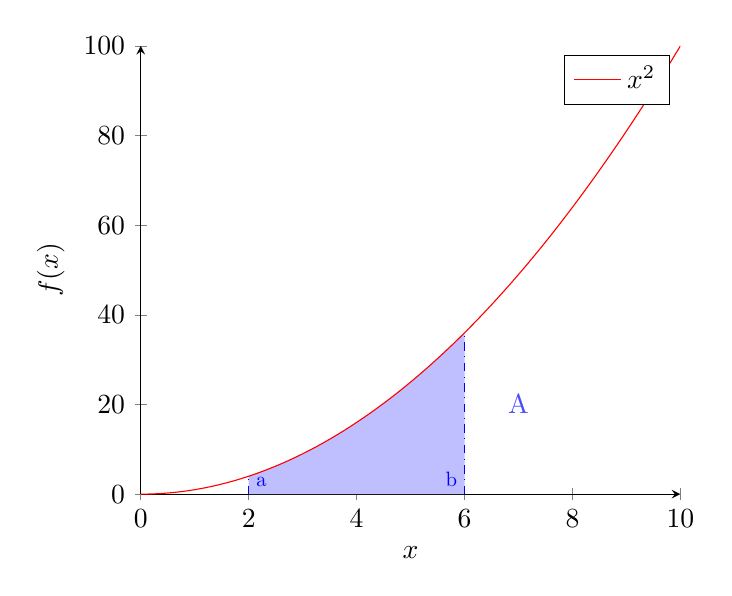
\begin{tikzpicture}
	\begin{axis}[
		axis lines = left,
		ylabel = $f(x)$,
		xlabel = $x$,
		]

		\path[name path=axis,] (axis cs:0,0) -- (axis cs:10,0);

		\addplot[name path = f, color=red, samples=1000, domain=0:10,]{x^2};
		\addlegendentry{$x^2$};

		\addplot[blue!25] fill between [
			of=f and axis,
			soft clip = {domain=2:6},
			];
		\node[blue!70] at (axis cs:7,20){A};

		\draw[dashdotted, blue] (axis cs:2,0) -- (axis cs:2,4);

		\draw[dashdotted, blue,] (axis cs:6,0) -- (axis cs:6,36);

		\node[blue, above right, scale=0.75] at (axis cs:2,0){a};

		\node[blue, above left, scale=0.75] at (axis cs:6,0){b};

	

	\end{axis}
\end{tikzpicture}
\end{center}
\bigbreak

\begin{equation}
A = \int^{b}_{a}f(x)\ dx = F(b) - F(a)
\end{equation}

\end{document}
